\chapter{Scenarii de utilizare }

In contextul actual al dezvoltarii tehnologice si adaptarii la era digitala, este nevoie de solutii moderne si eficiente din punctul de vedere al gestionarii resurselor, astfel incat sa tinem pasul cu avansul tehnologic si digital actual.

Platforma web AudIT ofera utilizatorilor sai diferite functionalitati care incearca sa rezolve probemele si sa ajute in procesul de audit public.

\section{Gestionarea misiunilor de audit}
\subsection*{Crearea unei misiuni de audit}
Pasul initial este crearea unei misiuni de audit noua, in care auditorul poate stabili parametri esentiali in alcatuirea unei noi misiuni de audit.

Procesul de creare a unei noi misiuni de audit public este astfel impartit in mai multi pasi:

\begin{itemize}
	\item   setarea numelui misiunii de audit, in care auditorul alege un nume descriptiv care sa reflecte aspectele cheie ale noii misiuni de audit creata. Numele ales este restrictionat de aplicatie astfel incat acesta poate contine doar litere si eventual cifre.
	
	\item  selectarea dintr-o lista a institutiei asupra caruia se efectueaza misiunea de audit;
	
	\item selectarea departamentului din cadrul institutiei astfel incat toate resursele create ulterior in cadrul acestei misiuni de audit o sa fie alocate eficient, fiind mai usor de preluat in pasii ce vor urma;
	
	\item in urma configurarii cu succes, auditorului ii este prezentat un dialog in care acesta poate revizui toti parametrii setati si sa confirme crearea unei noi misiuni de audit;
	
	Ulterior crearii unei noi misiuni de audit, utilizatorul este redirectionat catre pagina in care acesta poate vizualiza toate misiunile de audit create de el.
\end{itemize}

\subsection*{Alegerea misiunii de audit }
Utilizatorul poate vizualiza pe aceasta pagina toate misiunile de audit create de acesta si are posibilitatea de a selecta una dintre acestea pentru a vizualiza in detaliu informatii specifice pe pagina dedicata misiunii de audit. 

De asemenea, utilizatorul poate cauta in functie de nume o misiune de audit folosindu-se de bara de cautare a unei misiuni de audit disponibila in bara de navigare rapida din stanga ecranului.


\vspace{1cm}
\begin{figure}[h]
	\centering
	
	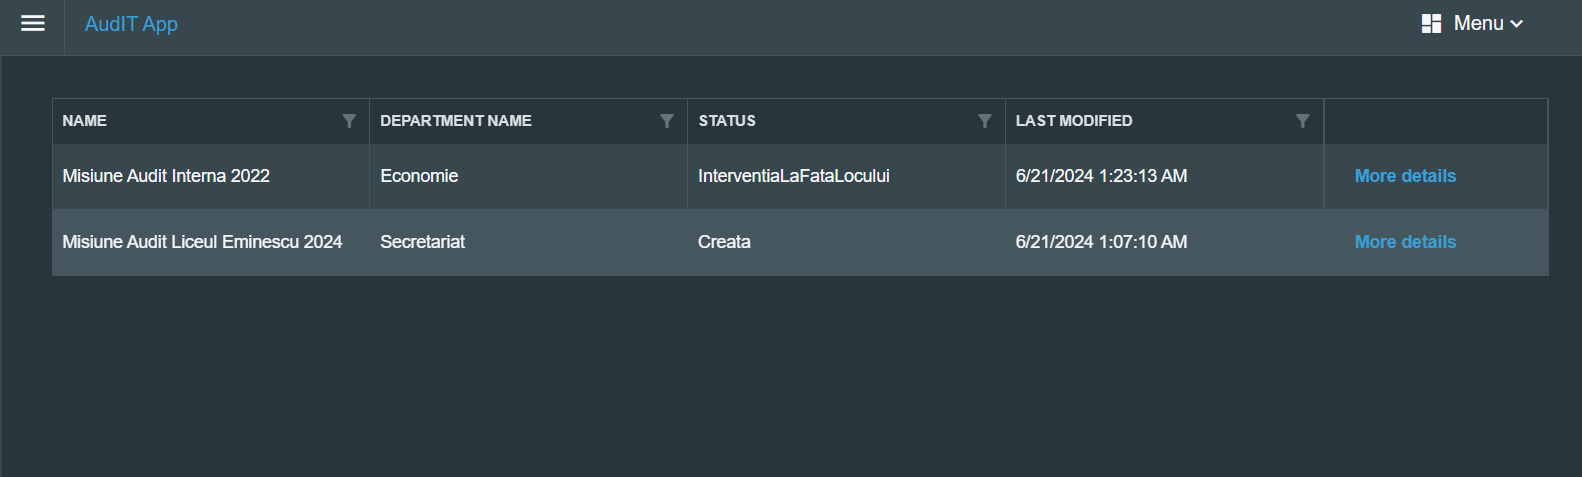
\includegraphics[width=1\textwidth]{c3/select_audit_mission.png}
	\caption{Selectarea misiunii de audit}
\end{figure}
\newpage
\subsection*{Selectarea misiunii de audit curente}
Pentru o eficienta mai buna in navigarea pe platforma, utilizatorul are optiunea de a selecta misiunea de audit curenta, astfel la majoritatea pasilor unde se cere selectarea unei misiuni de audit, alegerea implicita este misiunea de audit  curenta aleasa de utilizator.

In plus, un buton de navigare rapida spre pagina misiunii de audit curente este prezent in bara de navigare din stanga in sectiunea 'Audit Missions'.


\vspace{1cm}
\begin{figure}[h]
	\centering
	
	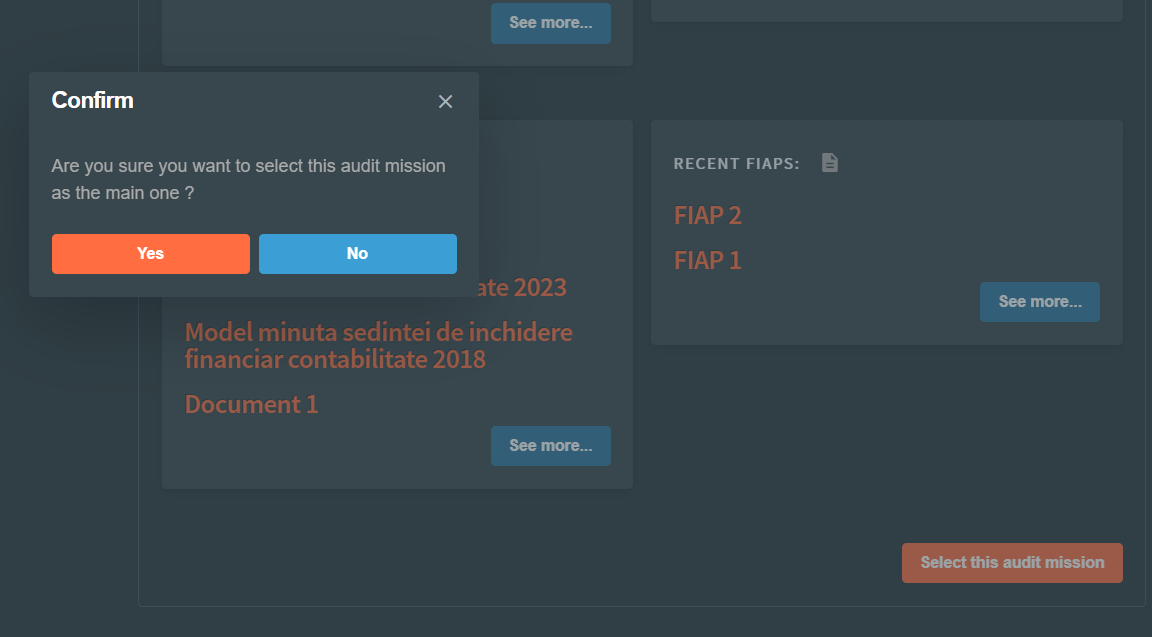
\includegraphics[width=0.7\textwidth]{c3/select_curren_audit.png}
	\caption{Selectarea misiunii de audit curente}
\end{figure}

\section{Gestionarea obiectivelor si a actiunilor}

\subsection*{Creare Obiectiv}
Auditorul poate intocmi noi obiective pe pagina dedicata acestei actiuni.La accesarea paginii, utilizatorului ii sunt prezentate o serie de pasi care in final vor rezulta in crearea unui nou obiectiv:

\begin{itemize}
	\item primul pas consta in selectarea unui nume respectiv a unei misiuni de audit pentru noul obiectiv;
	
	\item pasul secund ii ofera auditorului posibilitatea de a crea si atasa actiuni ce apartin noului obiectiv. Acesta trebuie sa specifice un numele noii actiuni, o lista de controale interne asteptate, o lista de controale interne existente respectiv daca actiunea o sa faca parte din procesul de auditare ulterior;
	
	\item al treilea pas permite  auditorului sa atasaze documentele intocmite deja de acesta in vederea crearii unui noi obiectiv. Acesta trebuie sa specifice tipul documentului pe care il incarca(document de sine statator sau document tip sablon), in cazul celei din urma optiuni, se specifica in plus versiunea documenutului, pasul la care este folosit acesta in cadrul misiunii de audit  si tipul documentului(\textit{draft}, \textit{published} sau \textit{archived}).
\end{itemize}

\vspace{1cm}
\begin{figure}[h]
	\centering
	
	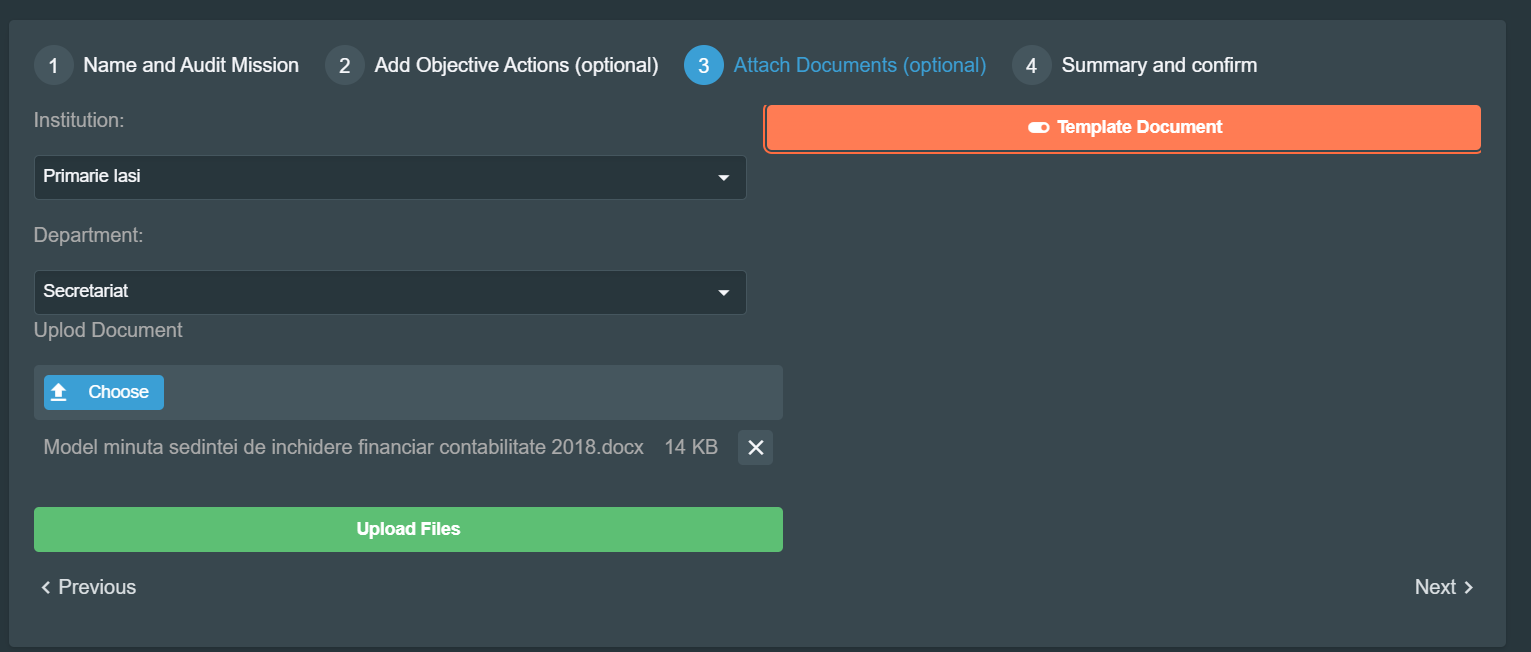
\includegraphics[width=1\textwidth]{c3/atach_document}
	\caption{Atasarea unui document la obiectivul nou creat}
\end{figure}


\subsection*{Vizualizare obiective}
Dupa crearea cu succes a unui nou obiectiv, utilizatorul este redirectionat catre pagina unde acesta poate vizualiza intr-un tabel toate obiectivele unei misiuni de audit selectate.

Fiecare linie din tabel prezinta un obiectiv, iar la apasarea pe respectiva linie, aceasta se mareste, astfel prezentand urmatoarele informatii utilizatorilor:
	\begin{itemize}
	
		\item un tabel care prezinta actiunile ce apartin obiectivului de pe linia selectata, afisand informatii precum nume, data ultimii modificari sau daca este selectat in procesul de auditare;
		
		\item un buton '\textit{More details}' care ofera navigare catre pagina dedicata vizualizarii actiunii selectata;
		
		\item o sectiune destinata setarilor asupra obiectivului selectat, unde utilizatorul poate modifica numele obiectivului sau optiunea de a sterge definitiv obiectivul respectiv;
		
		\item in partea inferioara a tabelului este prezent un buton '\textit{Add objective} care redirectioneaza utilizatorul la pagina dedicata crearii unui nou obiectiv.
		
	
	\end{itemize}


\vspace{1cm}
\begin{figure}[h]
	\centering
	
	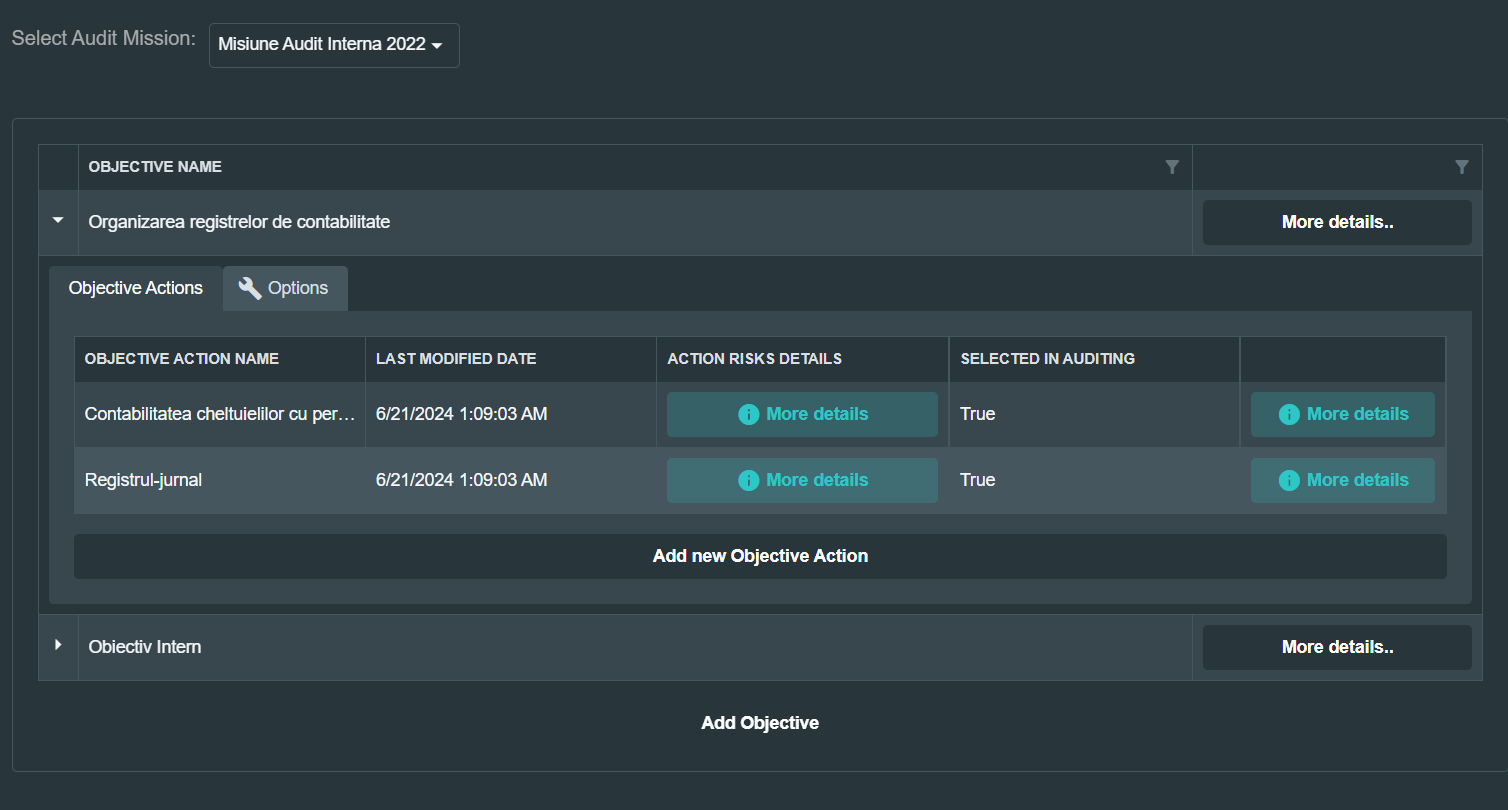
\includegraphics[width=1\textwidth]{c3/view_objective}
	\caption{Vizionarea obiectivelor asociate misiunii de audit}
\end{figure}



\subsection*{Identificarea si evaluarea riscuri}

Un pas esential in procesul de audit public il constituie identificarea si evalurea riscurilor actiunilor obiectivelor ce apartin unei misiuni de audit. Acest pas implica analiza si intelegerea riscurilor si ce implicatii si impact pot avea acestea.

 Platforma AudIT ofera auditorilor posibilitatea sa configureze riscuri si sa le actualizeze in functie de orice modificare poate aparea in procesul de audit public.
 
 Aceasta functionalitate este disponibila in mai multe pagini din aplicatie, astfel sporind eficienta cu care auditorii executa sarcini, facilitand o navigare mai usoara pe platforma.
 
 \subsection*{Vizualizare riscuri}
 Riscurile identifcate pot fi vizualizate pe pagina dedicata actiunii de care apartin, acestea putand fi sortate si filtrate dupa diferite caractestici cum ar fi: impactul acestora, scorul total sau alfabetic dupa numele acestora.
 
 \vspace{1cm}
 \begin{figure}[h]
 	\centering
 	
 	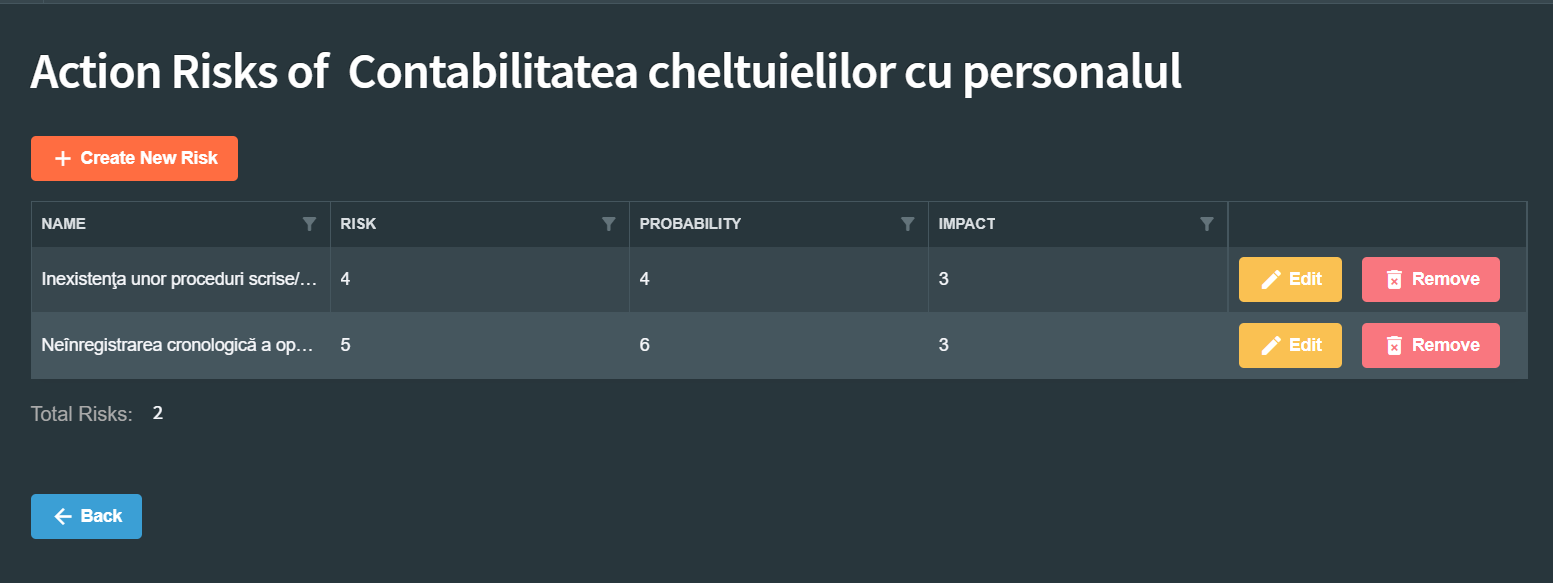
\includegraphics[width=1\textwidth]{c3/action_risks.png}
 	\caption{Vizualizarea riscurilor asociate actiunii}
 \end{figure}
 
 \subsection*{Gestionare riscuri}
Gestionarea riscurilor este de asemenea un pas esential in procesul de audit public, astfel, auditorul poate sa creeze noi riscuri si sa le actualizeze pe cele existente deja.

La apasarea butonului de 'Create new Risk', utilizatorului ii este prezentat un dialog in care acesta are posibiltiatea de completa proprietati ale noului risc: probabilitate, impact si scorul total al riscului. Dupa salvarea noului risc, tabelul este actualizat, iar utilizatorul poate vizualiza in acesta noua entitate creata.

\vspace{1cm}
\begin{figure}[h]
	\centering
	
	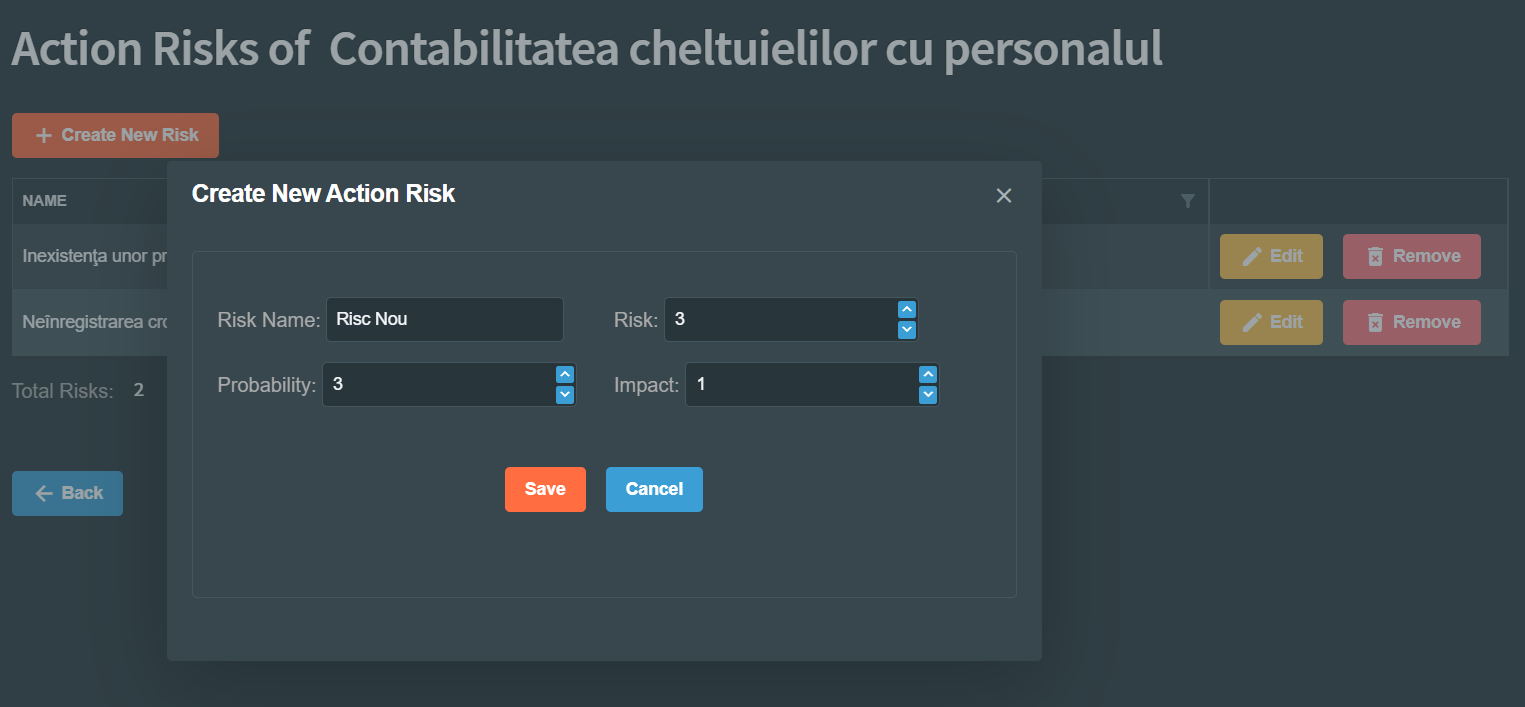
\includegraphics[width=1\textwidth]{c3/create_risk.png}
	\caption{Crearea unui risc nou}
\end{figure}


De asemenea, in partea inferioara a tabelului ,este afisat si un numarul total de riscuri asociate actiunii respective, pentru a oferi utilizatorului o idee asupra numarului de entitati de acest tip existente la momentul actual. 



\section{Gestionarea recomandarilor}

\subsection*{Creare recomandare}
La navigarea catre pagina dedicata crearii unei noi recomandari, utilizatorului ii sunt prezentate o serie de pasi care vor rezulta in crearea unei noi recomandari:
	
	\begin{itemize}
		\item primul pas consta in selectarea unui obiectiv pentru a tria actiunile prezente la pasul urmator;
		
		\item in al doilea pas se selecteaza actiunea asupra careia se va adauga noua recomandare;
		
		\item in cel de-al treilea pas, auditorul completeaza informatii specifice unei recomandari, cum ar fi : numele, problema adresata, data maxima de implementare, descrierea problemei, cauza si consecinte;
		
		\item in pasul final, utilizatorul trebuie sa confirme parametri setati si sa modifice erorile prezente in informatiile date.
	\end{itemize}


\newpage
\vspace{1cm}
\begin{figure}[h]
	\centering
	
	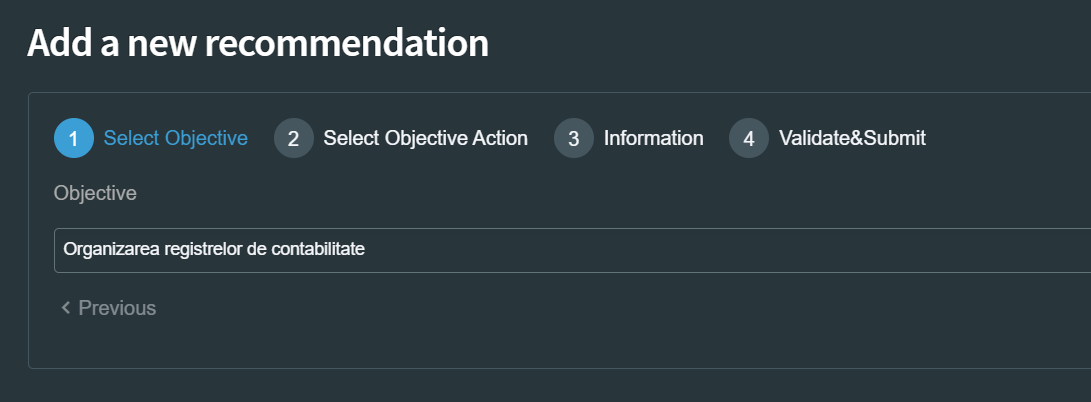
\includegraphics[width=1\textwidth]{c3/creare_recomandare1.png}
	\caption{Primul pas in crearea recomandarii}
\end{figure}

\vspace{1cm}
\begin{figure}[h]
	\centering
	
	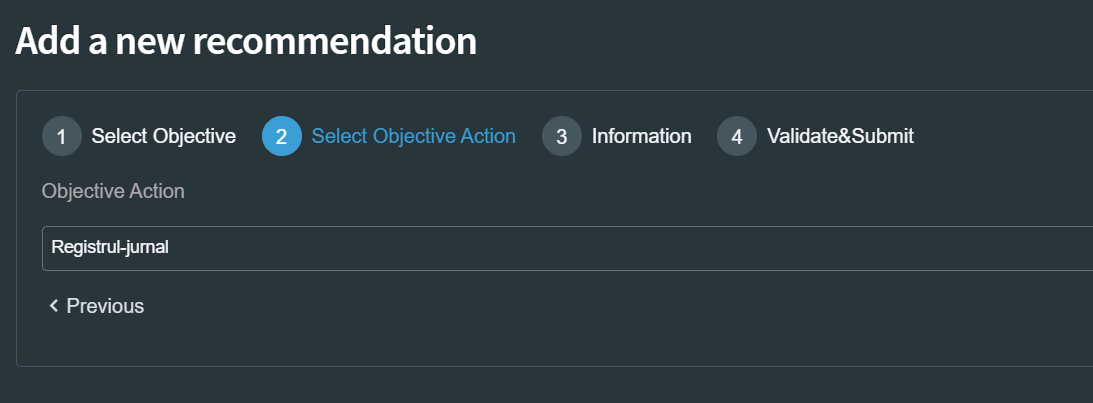
\includegraphics[width=1\textwidth]{c3/creare_recomandare2.png}
	\caption{Al doilea pas in crearea recomandarii}
\end{figure}

\vspace{1cm}
\begin{figure}[h]
	\centering
	
	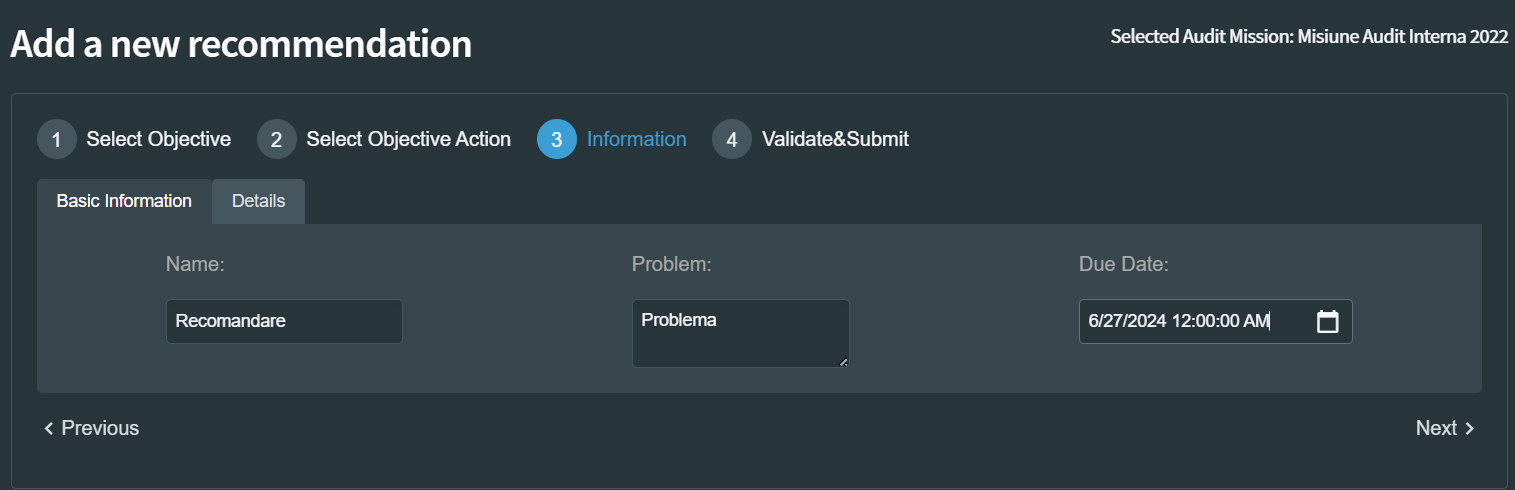
\includegraphics[width=1\textwidth]{c3/creare_recomandare3.png}
	\caption{Al treilea pas in crearea recomandarii}
\end{figure}

\newpage
\subsection*{Vizualizarea recomandarilor}

Dupa crearea cu succes a unei recomandari, utilizatorul este redirectionat catre pagina unde acesta poate vizualiza intr-un tabel toate recomandarile adaugate in misiunea de audit curenta.

Similar cu tabelul in care se vizualizeaza obiectivele, un rand prezinta numele recomandarii, statusul acesteia(daca este sau nu implementata) si data maxima pana cand aceasta trebuie implementata. La apasarea unui rand, acesta se mareste si utilizatorului ii sunt prezentate informatiile recomandarii cu posibilitatea ca acesta sa le modifice prin apasarea butonului '\textit{Edit}' urmat de '\textit{Confirm}' sau '\textit{Cancel}'.

De asemenea, in partea inferioara a tabelului este prezent un buton '\textit{Add new recommendation}' care il redirectioneaza pe utilizator pe pagina unde acesta poate crea o nouoa recomandare.

In plus, aceasta pagina, cu functionalitatea de editare a recomandarii restrictonata, le este disponbila in accesare si utilizatorilor de tipul reprezentantilor institutiilor, care trebuie sa verifice noile modificari si recomandari in misiunea de audit la care au acces.\\

\newpage
\vspace{1cm}
\begin{figure}[h]
	\centering
	
	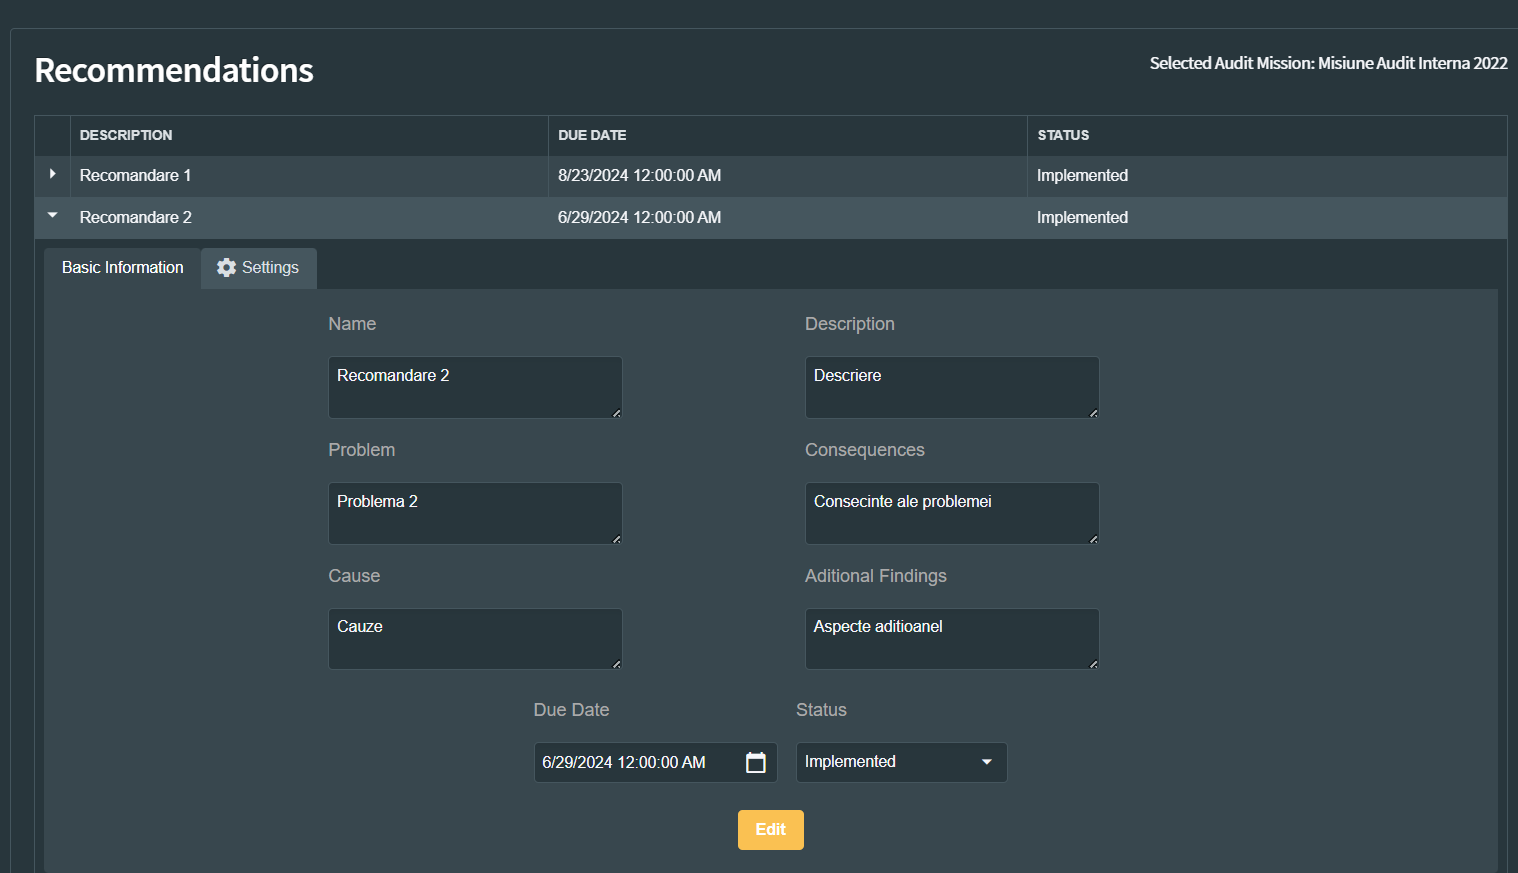
\includegraphics[width=1\textwidth]{c3/view_recommendations}
	\caption{Vizualizarea si editarea recomandarilor}
\end{figure}

\section{Gestionarea documentelor}

\subsection*{Salvarea documentelor pe platforma}

Utilizatorii au posibilitatea de a incarca pe platforma documente pentru o transparenta mai buna cat si o eficienta mai mare in distribuirea si accesarea informatiilor partajate.

Pagina de incarcare a unui document este structurata astfel incat utilizatorului ii sunt prezentati mai multi pasi care rezulta in incarcarea unui document pe platforma:
	
	\begin{itemize}
		\item  primul pas consta in selectarea institutiei careia ii este destinat documentul;
		
		\item pasul secund consta in selectarea departamentului din cadrul institutiei de la pasul anterior;
		
		\item ultimul pas presupune alegerea tipului documentului(de sine statator sau sablon) iar in cazul ultimii optiuni, utilizatorul trebuie sa specifice versiunea, pasul din cadrul misiunii de audit corespunzator documentului respectiv tipul acestuia, urmand ca ulterior la apsarea butonului '\textit{Choose}' ,utilizatorul sa selecteze un document din fisierele sale si sa il incarce pe platforma.
		
		
	\end{itemize}


\vspace{1cm}
\begin{figure}[h]
	\centering
	
	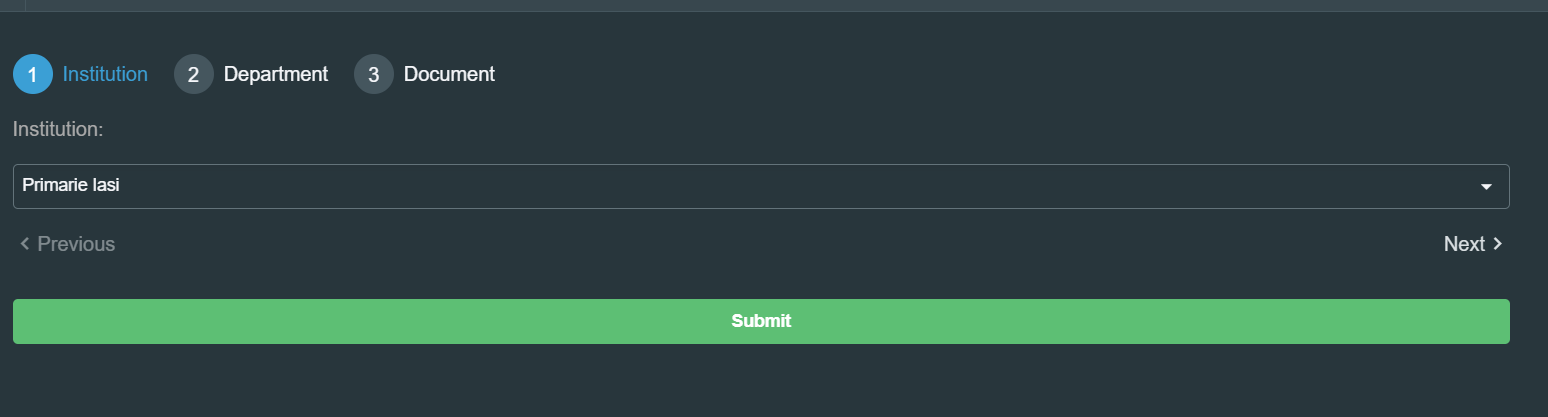
\includegraphics[width=1\textwidth]{c3/creare_document1.png}
	\caption{Primul pas in incarcarea documentului}
\end{figure}


\vspace{1cm}
\begin{figure}[h]
	\centering
	
	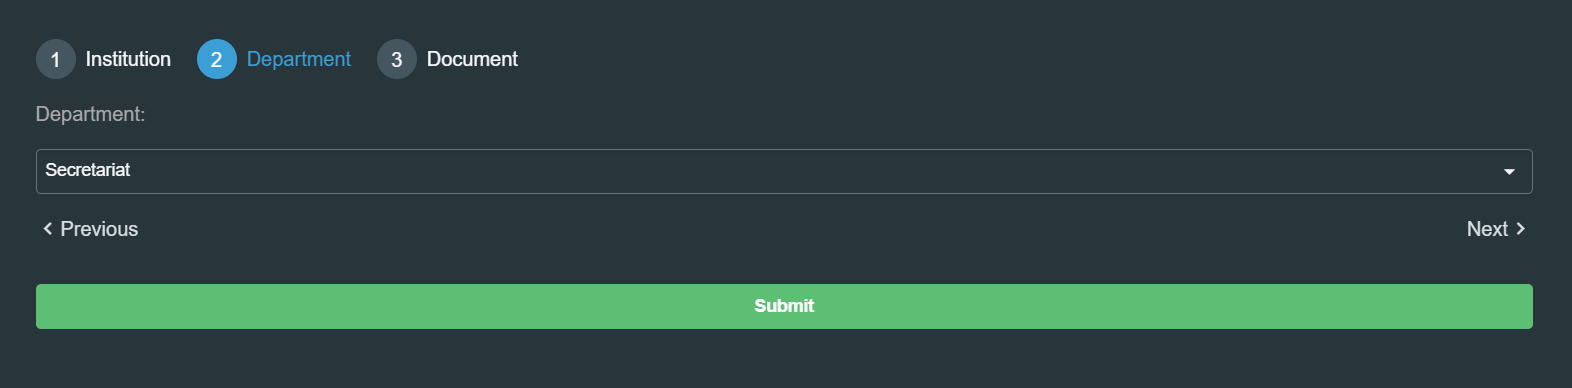
\includegraphics[width=1\textwidth]{c3/creare_document2.png}
	\caption{Al doilea pas in incarcarea documentului}
\end{figure}


\vspace{1cm}
\begin{figure}[h]
	\centering
	
	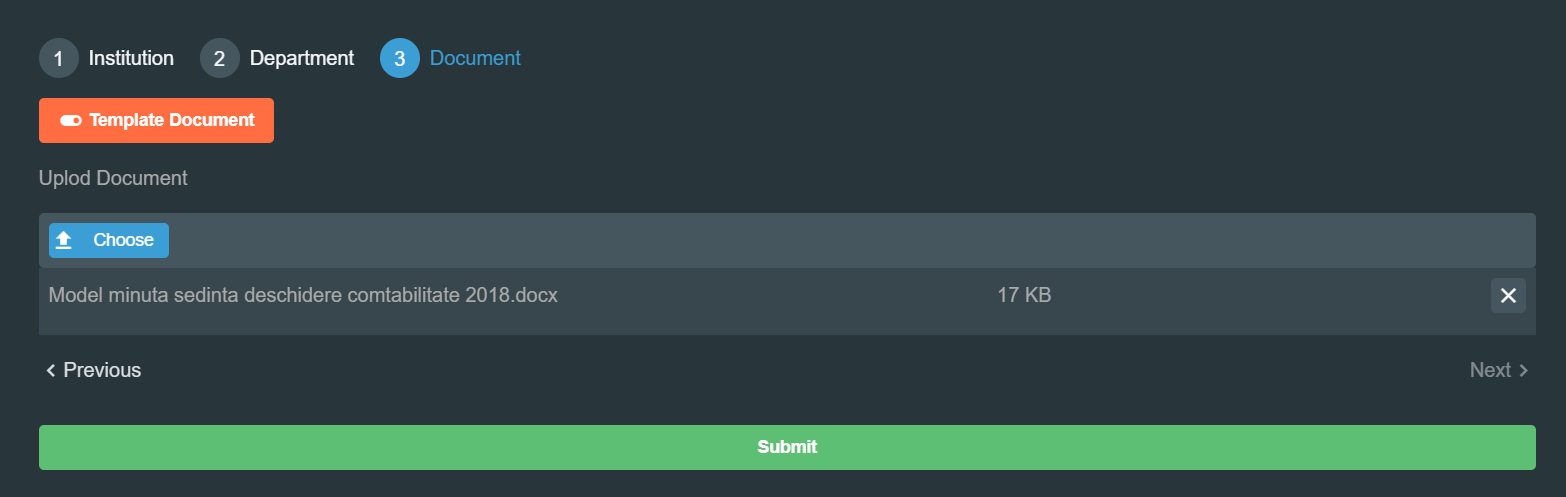
\includegraphics[width=1\textwidth]{c3/creare_document3.png}
	\caption{Al treilea pas in incarcarea documentului}
\end{figure}

\subsection*{Vizualizarea documentelor}

Vizualizarea documentelor se face pe pagina dedicata vizualizarii, accesibila prin apasarea butonului
'\textit{List Documents}' din bara de navigare rapida.

Documentele utilizatorului sunt dispuse intr-un tabel, afisand informatii precum ar fi: numele documentului, extensia si tipul acestuia.


\vspace{1cm}
\begin{figure}[h]
	\centering
	
	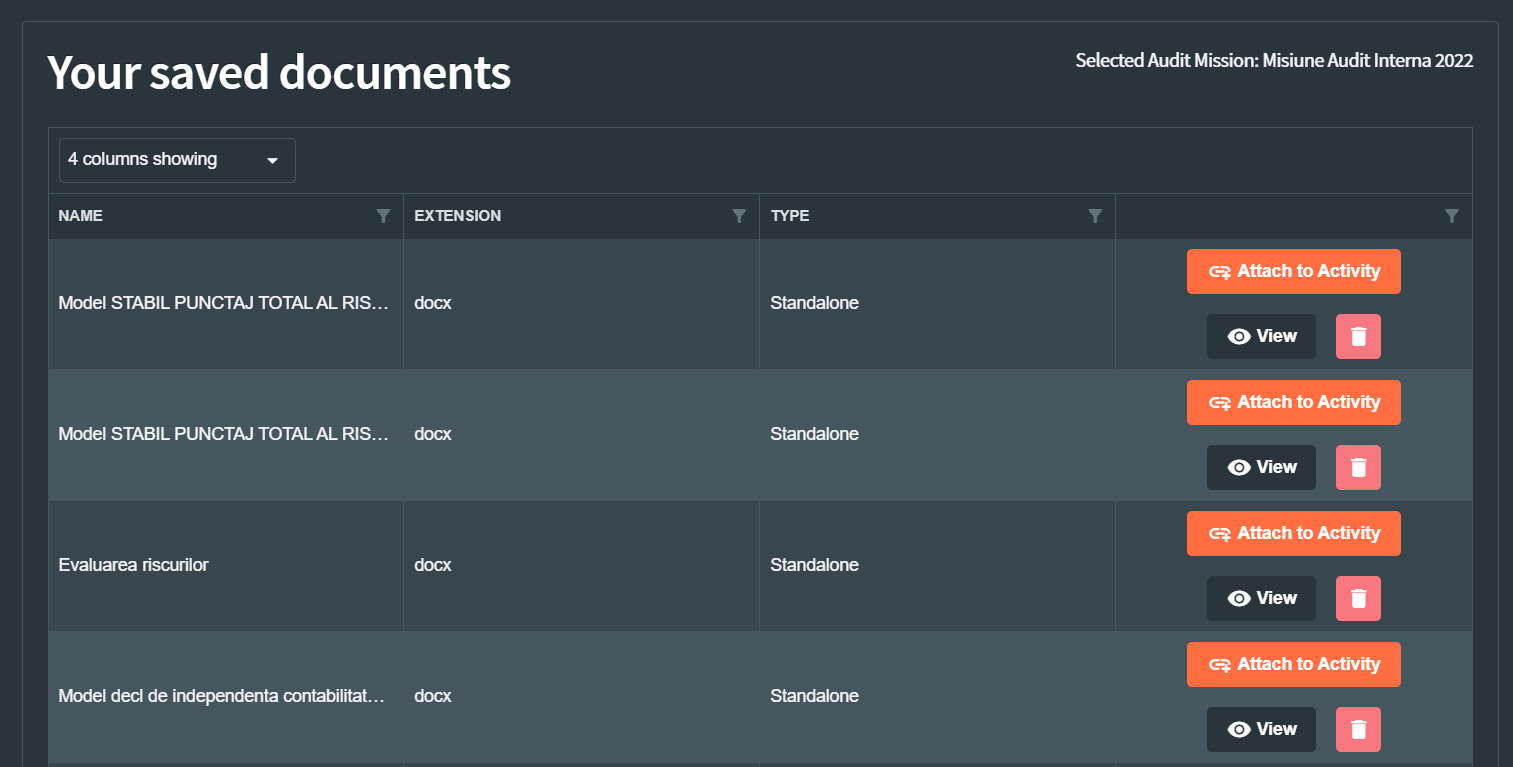
\includegraphics[width=1\textwidth]{c3/view_documents.png}
	\caption{Vizualizarea documentelor }
\end{figure}


De asemenea, utilizatorul are posibilitatea de a atasa documentul la o activitate, de a vizualiza documentul in cazul unui document de sine statatot, transformand-ul in format PDF, de a edita documentul direct pe platforma in cazul in care documentul este unul de tip sablon sau optiunea de a sterge documentul din stocarea platformei.\\


\vspace{1cm}
\begin{figure}[h]
	\centering
	
	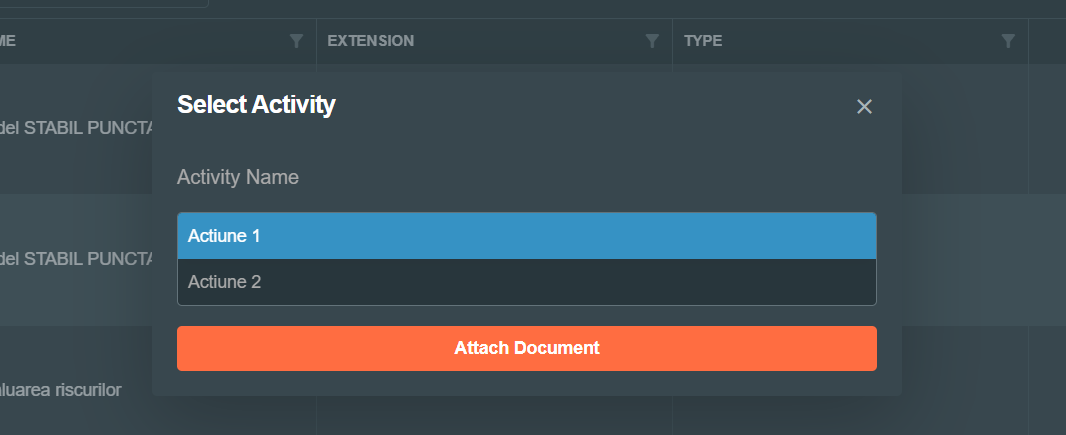
\includegraphics[width=1\textwidth]{c3/attach_document_to_activity.png}
	\caption{Atasarea unui document la o activitate selectata}
\end{figure}



\section{Sistemul de export}

Sistemul de export este proiectat avand ca functionalitate principala transferul informatiilor care se afla pe platforma catre diferite formate, cum ar fi : XLSX, DOCS ,precum si in autocompletarea unor documente oficiale de tip sablon pe care auditorul are obligatia sa le completeze in decursul unei misiuni de audit.

Utilizatorii au astfel posibilitatea sa utilizeze acest sistem in mai multe feluri:
\subsection*{Exportare activitati}
Utilizatorul are optiunea de a exporta activitatile inregistrate pe platforma in format CSV prin navigarea pe pagina de \textit{Export Activities} prin apasarea butonului respectiv.

Pagina este compusa din doua tabele, utilizatorul putand sa selecteze actiunile care doreste sa le salveze din tabelul din partea stanga, activitatile selectate fiind afisate in tabelul din partea dreapta.

La apasarea butonului de '\textit{Export}', acesta poate descarca fisierul cu extensia .CSV, avand optiunea ca ulterior sa il salveze pe platforma ca un document de sine statator.


\vspace{1cm}
\begin{figure}[h]
	\centering
	
	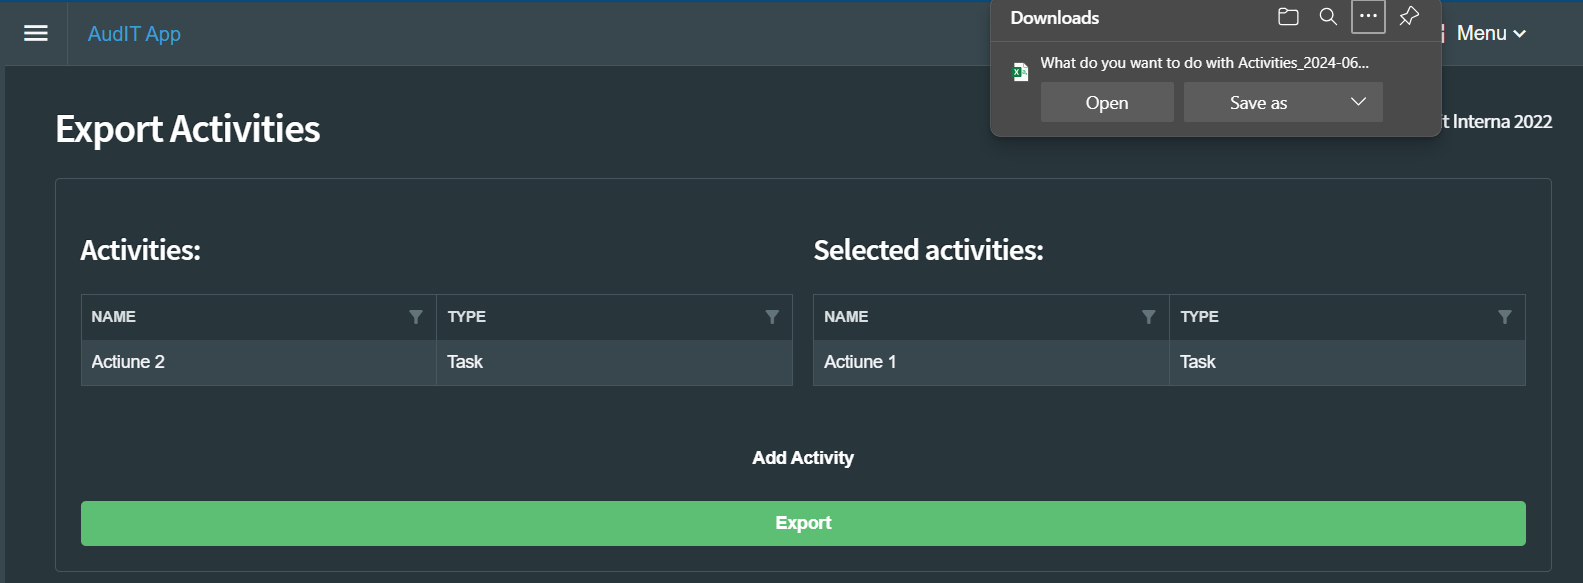
\includegraphics[width=1\textwidth]{c3/export_activities.png}
	\caption{Exportarea activitatilor in format .CSV}
\end{figure}

\subsection*{Exportare obiective si activitati}
La apasarea butonului '\textit{Export Objectives and Risks}' din bara de navigare din stanga, utilizatorului ii este prezentat un dialog in care acesta selecteaza misiunea de audit asupra careia doreste sa efectueze actiunea de export. Din aceasta, sunt selectate toate obiectivele si actiunile cu riscurile corespunzatoare si se autocompleteaza un document tip sablon oficial cu datele selectate. Ulterior completarii, utilizatorul poate sa descarce documentul generat pe platforma, avand ulterior similar posibilitatea de a il salva pe platforma. 


\vspace{1cm}
\begin{figure}[h]
	\centering
	
	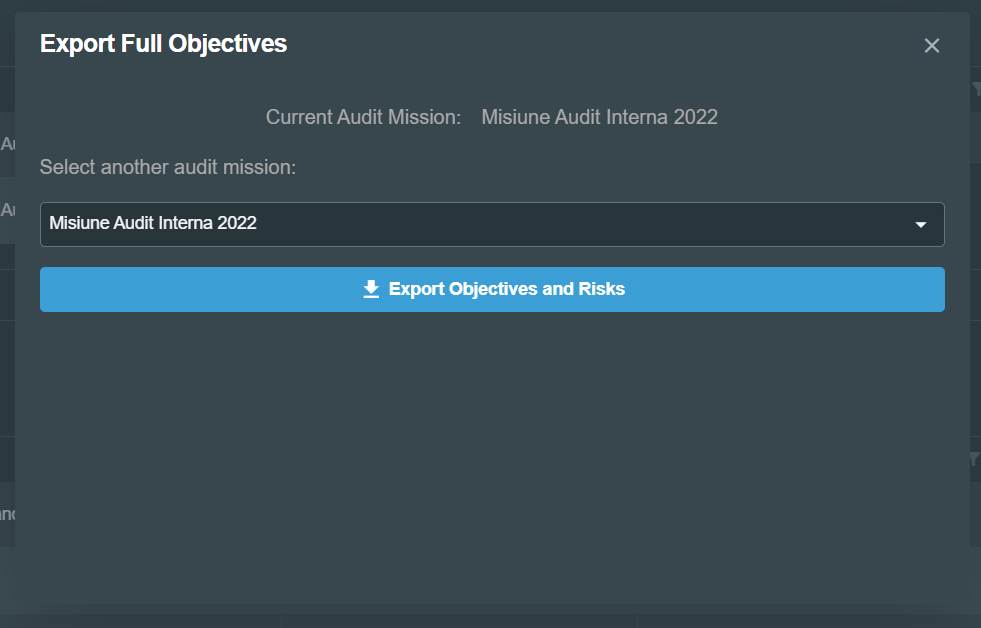
\includegraphics[width=1\textwidth]{c3/export_objectives.png}
	\caption{Exportarea obiectivelor si a actiunilor }
\end{figure}


\vspace{1cm}
\begin{figure}[h]
	\centering
	
	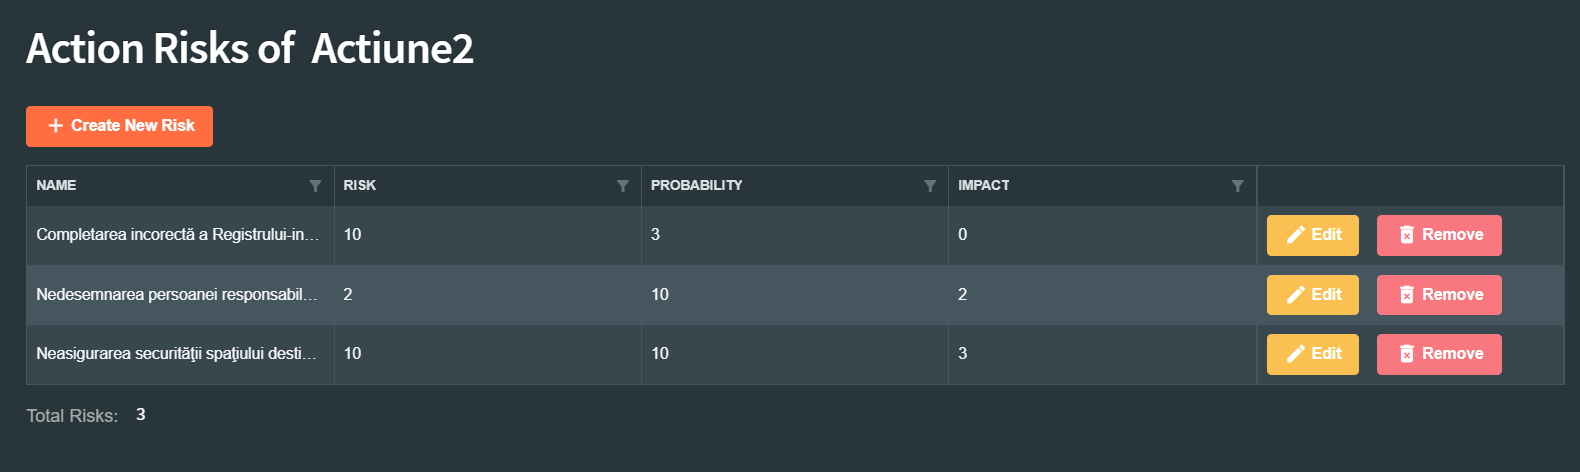
\includegraphics[width=1\textwidth]{c3/tabel_riscuri.png}
	\caption{Documentul autocompletat}
\end{figure}


\subsection*{Autocompletare FIAP}
Auditorul are posibilitatea de a autocompleta un document tip sablon FIAP (Fisa Identificare si Analiza a Problemei) prin acesarea paginii de '\textit{Export FIAP}'.

Pagina contine un tabel in care sunt prezente toate recomandarile facute de auditor in cadrul misiunii de audit specificate, acesta avand posibilitatea de a selecta un rand din tabel si a apasa pe butonul '\textit{Autocomplete\&Download}' pentru a autocompleta automat documentul cu datele recomandarii si a il descarca pe propriul \textit{computer}.


\vspace{1cm}
\begin{figure}[h]
	\centering
	
	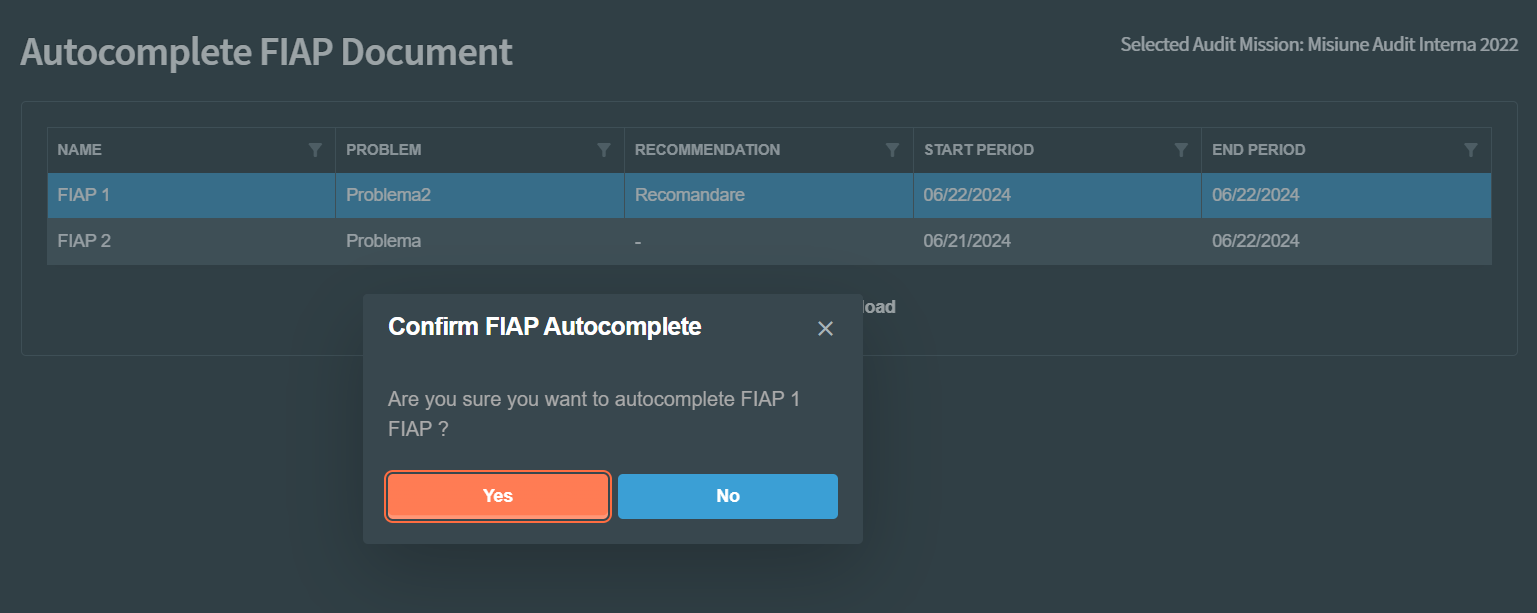
\includegraphics[width=1\textwidth]{c3/export_fiap.png}
	\caption{Exportarea documentului FIAP}
\end{figure}

\vspace{1cm}
\begin{figure}[h]
	\centering
	
	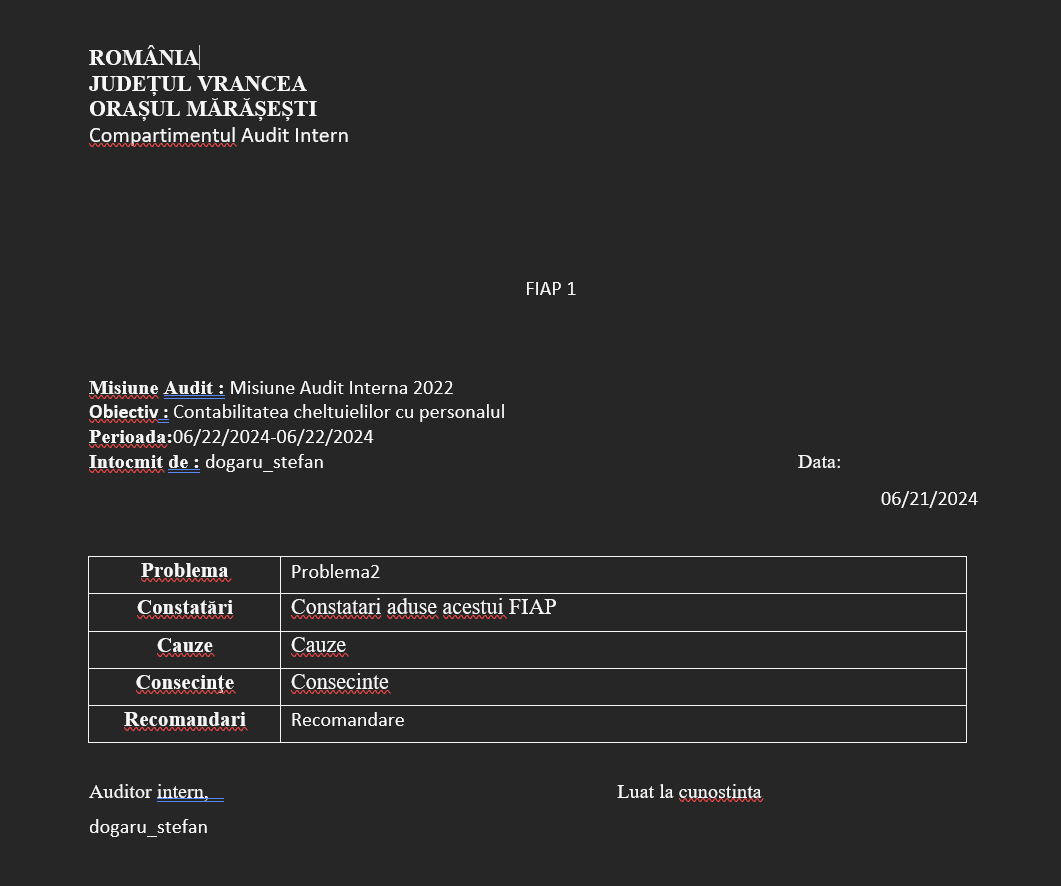
\includegraphics[width=1\textwidth]{c3/document_FIAP}
	\caption{Documentul FIAP autocompletat}
\end{figure}

 


